\documentclass[border=10pt]{standalone}
% Shared preamble for the README figures. Build with `docs/figures/build.sh`.
\usepackage[T1]{fontenc}
\usepackage{libertinus}
\setmonofont{Inconsolatazi4-Regular.otf}[Scale=0.86,BoldFont=Inconsolatazi4-Bold.otf]
\usepackage{amsmath}
\usepackage{tikz}
\usepackage{pgfplots}
\pgfplotsset{compat=1.18}
\usetikzlibrary{arrows.meta,positioning,calc,fit,backgrounds,decorations.pathreplacing,shapes.geometric,patterns}

\definecolor{ink}{gray}{0.11}
\definecolor{mute}{gray}{0.40}
\definecolor{faint}{gray}{0.62}
\definecolor{rule}{gray}{0.80}
\definecolor{fill}{gray}{0.955}
\definecolor{neg}{RGB}{164,38,44}
\definecolor{negfill}{RGB}{247,229,228}
\pagecolor{white}
\color{ink}

\tikzset{
  >={Stealth[length=5pt,width=4pt]},
  every picture/.style={line width=0.55pt, draw=ink},
  panel/.style={draw=rule, line width=0.6pt, fill=white},
  box/.style={draw=ink, fill=white, inner sep=3pt, font=\footnotesize},
  soft/.style={draw=rule, fill=fill, inner sep=3pt, font=\footnotesize},
  lab/.style={font=\footnotesize\color{mute}, inner sep=0pt},
  flow/.style={->, draw=ink, line width=0.7pt},
  code/.style={draw=rule, fill=fill, align=left, inner sep=4pt, font=\ttfamily\scriptsize, execute at begin node={\hyphenpenalty=10000\relax\exhyphenpenalty=10000\relax}},
}
\newcommand{\plabel}[2]{\textbf{(#1)}\,\textsc{#2}}

% Data: TRAIL GAIA trace 0140b3f657eddf76ca82f72c49ac8e58; judge run
% turn-judge-0044b8f5c041155c; verifier family-verifier-dadbdfb15ac3d641;
% scores verifier-scores-2e4d12bf28744e29 (checks only, no judge).
\begin{document}
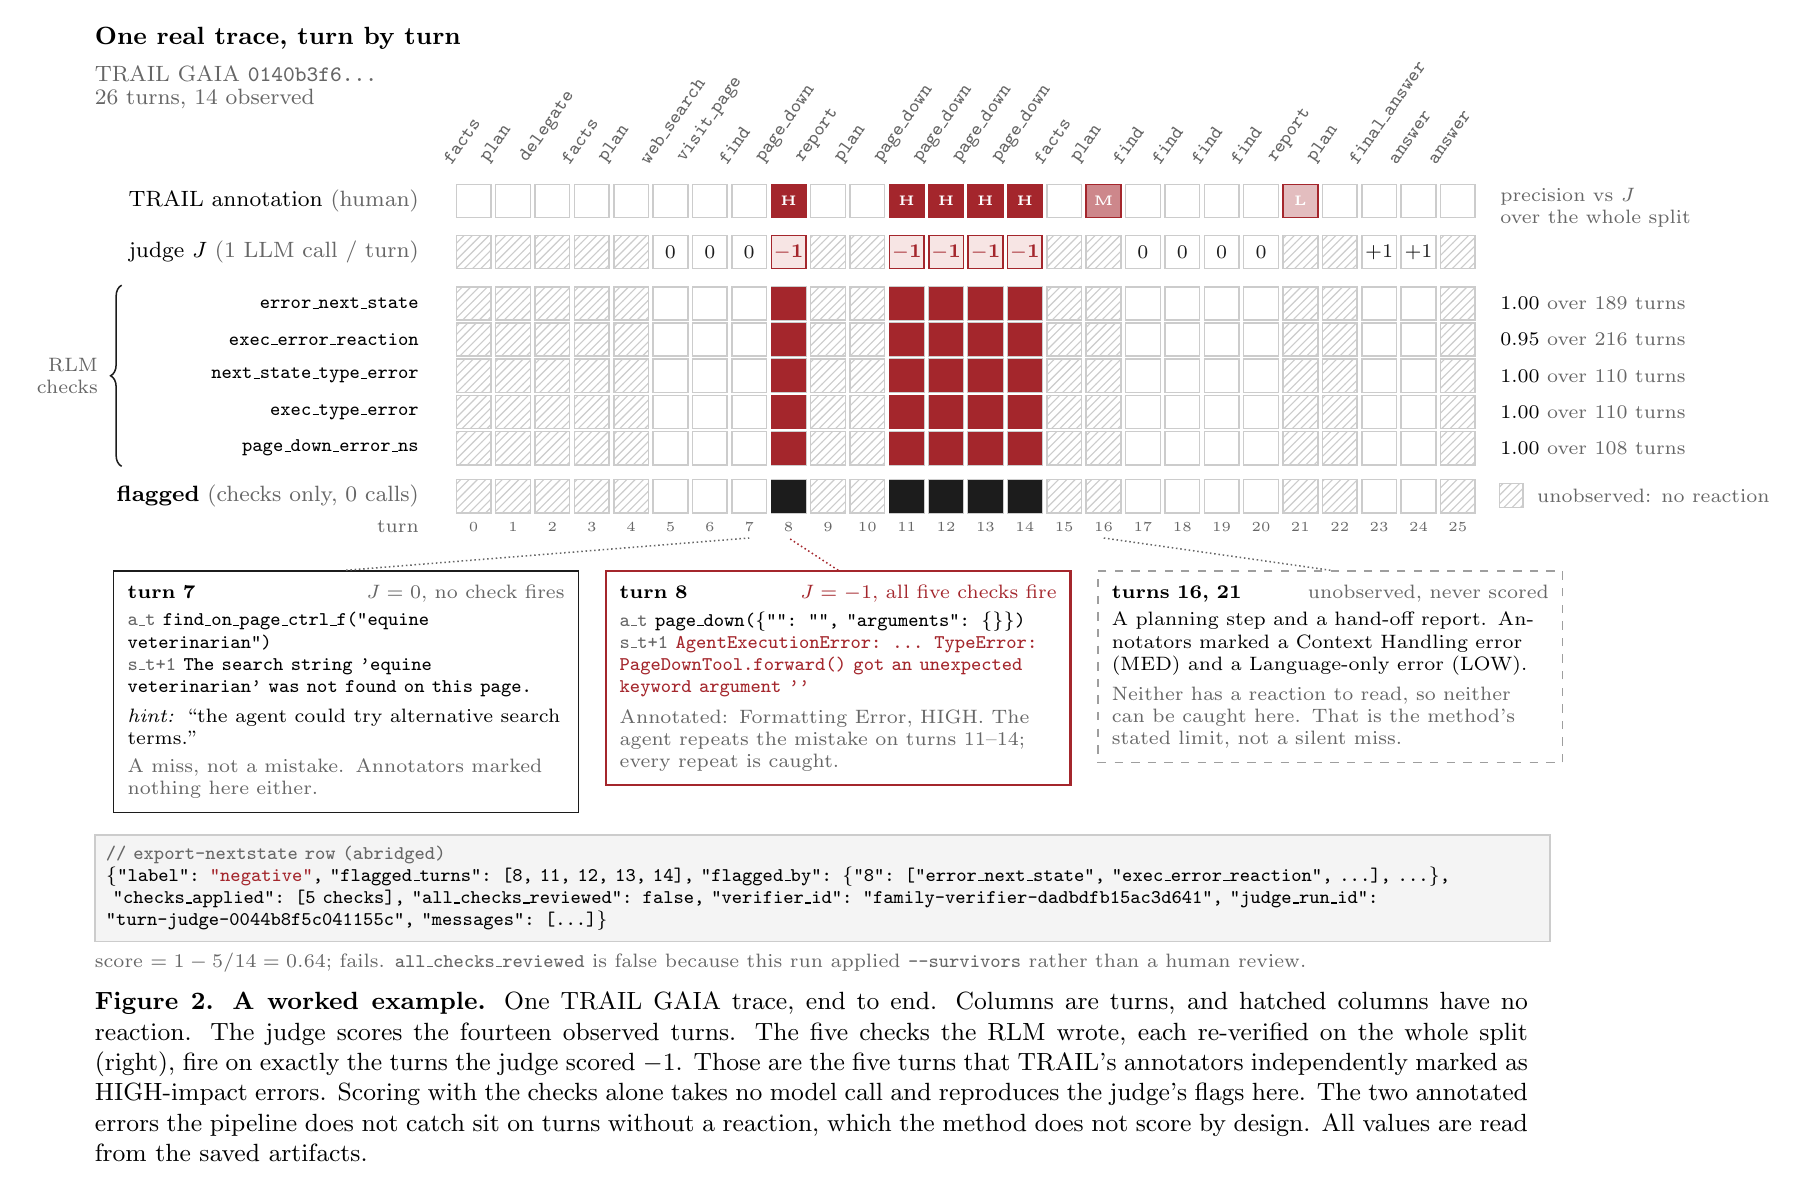
\begin{tikzpicture}[x=1cm,y=1cm]
\def\cw{0.5}   % cell width
\def\ch{0.42}  % cell height
\def\xo{4.6}   % x of turn 0
\newcommand{\cx}[1]{\xo+\cw*#1}

% unobserved turns
\def\unobs{0,1,2,3,4,9,10,15,16,21,22,25}
\def\neg{8,11,12,13,14}

% ---------- column labels (actions) ----------
\foreach \t/\a in {0/facts,1/plan,2/delegate,3/facts,4/plan,5/web\_search,6/visit\_page,7/find,8/page\_down,9/report,10/plan,11/page\_down,12/page\_down,13/page\_down,14/page\_down,15/facts,16/plan,17/find,18/find,19/find,20/find,21/report,22/plan,23/final\_answer,24/answer,25/answer}{
  \node[rotate=55, anchor=south west, font=\ttfamily\scriptsize, text=mute, inner sep=1pt] at (\cx{\t}-0.05,0.08) {\a};
}
\node[anchor=south west, font=\small\bfseries, inner sep=0] at (0,1.6) {One real trace, turn by turn};
\node[anchor=south west, font=\footnotesize, text=mute, inner sep=0] at (0,1.2) {TRAIL GAIA \texttt{0140b3f6\dots}};
\node[anchor=south west, font=\footnotesize, text=mute, inner sep=0] at (0,0.85) {26 turns, 14 observed};

% ---------- rows ----------
% row y positions (top of each row)
\def\yA{-0.1}  % annotation
\def\yJ{-0.75} % judge
\def\yC{-1.4}  % first check
\def\yV{-3.85} % verifier
\node[anchor=east, font=\footnotesize, align=right] at (\xo-0.35,\yA-\ch/2) {TRAIL annotation \textcolor{mute}{(human)}};
\node[anchor=east, font=\footnotesize] at (\xo-0.35,\yJ-\ch/2) {judge $J$ \textcolor{mute}{(1 LLM call / turn)}};
\foreach \n [count=\i from 0] in {error\_next\_state, exec\_error\_reaction, next\_state\_type\_error, exec\_type\_error, page\_down\_error\_ns}{
  \node[anchor=east, font=\ttfamily\scriptsize] at (\xo-0.35,\yC-\i*0.46-\ch/2) {\n};
}
\draw[decorate, decoration={brace, amplitude=4pt, mirror}] (0.35,\yC+0.02) -- (0.35,\yC-4*0.46-\ch-0.02) node[midway, left=5pt, font=\scriptsize, text=mute, align=right]{RLM\\checks};
\node[anchor=east, font=\footnotesize] at (\xo-0.35,\yV-\ch/2) {\textbf{flagged} \textcolor{mute}{(checks only, 0 calls)}};

% grid background + unobserved hatching
\foreach \t in {0,...,25}{
  \foreach \y in {\yJ,\yC,\yC-0.46,\yC-0.92,\yC-1.38,\yC-1.84,\yV}{
    \draw[draw=rule, fill=white] (\cx{\t},\y) rectangle ++(\cw-0.06,-\ch);
  }
  \draw[draw=rule, fill=white] (\cx{\t},\yA) rectangle ++(\cw-0.06,-\ch);
}
\foreach \t in \unobs{
  \foreach \y in {\yJ,\yC,\yC-0.46,\yC-0.92,\yC-1.38,\yC-1.84,\yV}{
    \fill[pattern=north east lines, pattern color=rule] (\cx{\t},\y) rectangle ++(\cw-0.06,-\ch);
  }
}
% annotations (impact)
\foreach \t/\imp/\op in {8/H/1,11/H/1,12/H/1,13/H/1,14/H/1,16/M/0.55,21/L/0.3}{
  \draw[draw=neg, fill=neg, fill opacity=\op] (\cx{\t},\yA) rectangle ++(\cw-0.06,-\ch);
  \node[font=\tiny\bfseries, text=white] at (\cx{\t}+\cw/2-0.03,\yA-\ch/2) {\imp};
}
% judge verdicts
\foreach \t/\v in {5/0,6/0,7/0,17/0,18/0,19/0,20/0,23/+1,24/+1}{
  \node[font=\scriptsize, text=ink] at (\cx{\t}+\cw/2-0.03,\yJ-\ch/2) {\v};
}
\foreach \t in \neg{
  \draw[draw=neg, fill=negfill] (\cx{\t},\yJ) rectangle ++(\cw-0.06,-\ch);
  \node[font=\scriptsize\bfseries, text=neg] at (\cx{\t}+\cw/2-0.03,\yJ-\ch/2) {$-$1};
}
% checks and verifier
\foreach \t in \neg{
  \foreach \y in {\yC,\yC-0.46,\yC-0.92,\yC-1.38,\yC-1.84}{
    \fill[neg] (\cx{\t},\y) rectangle ++(\cw-0.06,-\ch);
  }
  \fill[ink] (\cx{\t},\yV) rectangle ++(\cw-0.06,-\ch);
}
% turn index row
\foreach \t in {0,...,25}{
  \node[font=\tiny, text=mute] at (\cx{\t}+\cw/2-0.03,\yV-\ch-0.18) {\t};
}
\node[anchor=east, font=\scriptsize, text=mute] at (\xo-0.35,\yV-\ch-0.18) {turn};

% precision column
\def\xp{\xo+26*\cw+0.25}
\node[anchor=south west, font=\scriptsize, text=mute, align=left, inner sep=0] at (\xp,\yJ+0.1) {precision vs $J$\\over the whole split};
\foreach \p/\n [count=\i from 0] in {1.00/189, 0.95/216, 1.00/110, 1.00/110, 1.00/108}{
  \node[anchor=west, font=\scriptsize, inner sep=0] at (\xp,\yC-\i*0.46-\ch/2) {\p\ \textcolor{mute}{over \n\ turns}};
}

% legend
\begin{scope}[shift={(\xp,\yV-0.05)}]
  \draw[draw=rule, fill=white] (0,0) rectangle ++(0.3,-0.3); \fill[pattern=north east lines, pattern color=rule] (0,0) rectangle ++(0.3,-0.3);
  \node[anchor=west, font=\scriptsize, text=mute] at (0.35,-0.15) {unobserved: no reaction};
\end{scope}

% ---------- callouts ----------
\def\yb{-5.0}
\tikzset{call/.style={draw=ink, fill=white, align=left, text width=5.55cm, inner sep=5pt, anchor=north, font=\scriptsize}}
\node[call] (k7) at (3.2,\yb) {%
  \textbf{turn 7}\hfill\textcolor{mute}{$J=0$,\ no check fires}\\[2pt]
  \texttt{\textcolor{mute}{a\_t} find\_on\_page\_ctrl\_f("equine veterinarian")}\\
  \texttt{\textcolor{mute}{s\_t+1} The search string 'equine veterinarian' was not found on this page.}\\[3pt]
  \textit{hint:} ``the agent could try alternative search terms.''\\[2pt]
  \textcolor{mute}{A miss, not a mistake. Annotators marked nothing here either.}};
\node[call, draw=neg, line width=0.8pt] (k8) at (9.45,\yb) {%
  \textbf{turn 8}\hfill\textcolor{neg}{$J=-1$,\ all five checks fire}\\[2pt]
  \texttt{\textcolor{mute}{a\_t} page\_down(\{"": "", "arguments": \{\}\})}\\
  \texttt{\textcolor{mute}{s\_t+1} \textcolor{neg}{AgentExecutionError: ... TypeError: PageDownTool.forward() got an unexpected keyword argument ''}}\\[3pt]
  \textcolor{mute}{Annotated: Formatting Error, HIGH. The agent repeats the mistake on turns 11--14; every repeat is caught.}};
\node[call, draw=faint, dashed] (k16) at (15.7,\yb) {%
  \textbf{turns 16, 21}\hfill\textcolor{mute}{unobserved, never scored}\\[2pt]
  A planning step and a hand-off report. Annotators marked a Context Handling error (MED) and a Language-only error (LOW).\\[3pt]
  \textcolor{mute}{Neither has a reaction to read, so neither can be caught here. That is the method's stated limit, not a silent miss.}};
\draw[mute, densely dotted] (k7.north) -- (\cx{7}+\cw/2-0.03,\yV-\ch-0.32);
\draw[neg, densely dotted] (k8.north) -- (\cx{8}+\cw/2-0.03,\yV-\ch-0.32);
\draw[mute, densely dotted] (k16.north) -- (\cx{16}+\cw/2-0.03,\yV-\ch-0.32);

% ---------- export row ----------
\node[code, anchor=north west, text width=18.2cm, font=\ttfamily\scriptsize] (row) at (0.0,-8.35) {%
\textcolor{mute}{// export-nextstate row (abridged)}\\
\{"label": \textcolor{neg}{"negative"}, "flagged\_turns": [8, 11, 12, 13, 14],
 "flagged\_by": \{"8": ["error\_next\_state", "exec\_error\_reaction", ...], ...\},\\
\ "checks\_applied": [5 checks], "all\_checks\_reviewed": false, "verifier\_id": "family-verifier-dadbdfb15ac3d641",
 "judge\_run\_id": "turn-judge-0044b8f5c041155c", "messages": [...]\}};
\node[anchor=north west, font=\scriptsize, text=mute, inner sep=0] at ($(row.south west)+(0,-0.12)$) {score $=1-5/14=0.64$; fails. \texttt{all\_checks\_reviewed} is false because this run applied \texttt{--survivors} rather than a human review.};

% ---------- caption ----------
\node[anchor=north west, text width=18.2cm, align=justify, font=\small, inner sep=0] at (0,-10.35) {%
\textbf{Figure 2.} \textbf{A worked example.} One TRAIL GAIA trace, end to end. Columns are turns, and hatched columns have no reaction. The judge scores the fourteen observed turns. The five checks the RLM wrote, each re-verified on the whole split (right), fire on exactly the turns the judge scored $-1$. Those are the five turns that TRAIL's annotators independently marked as HIGH-impact errors. Scoring with the checks alone takes no model call and reproduces the judge's flags here. The two annotated errors the pipeline does not catch sit on turns without a reaction, which the method does not score by design. All values are read from the saved artifacts.};

\end{tikzpicture}
\end{document}
